\documentclass[11pt]{article}
\usepackage[english]{babel}
\usepackage{geometry}
\usepackage{amsmath}
\usepackage{amsthm}
\usepackage{graphicx}
\usepackage{caption}
\usepackage[utf8]{inputenc}


%%%%%%%% SUB-FIGURE PACKAGE
\usepackage{subcaption}

%%%%%%%% MULTI-COLUMNS PACKAGE
\usepackage{multicol}

%%%%%%%% PERSONAL COMMANDS
\usepackage{amssymb}

%%%% Important sets
\renewcommand{\O}{\mathbb{O}}
\newcommand{\N}{\mathbb{N}}
\newcommand{\Z}{{\mathbb{Z}}}
\newcommand{\Q}{{\mathbb{Q}}}
\newcommand{\R}{{\mathbb{R}}}

%%%% Usual operations
\newcommand{\pow}[2]{#1^{#2}}
\newcommand{\expp}[1]{e^{#1}}
\newcommand{\fst}{\mathrm{fst}}
\newcommand{\snd}{\mathrm{snd}}

%%%% Lambda Calculus
\newcommand{\dneq}{\,\, \# \,\,}
\newcommand{\prm}[1]{\pmb{\mathrm{#1}}}
\renewcommand{\S}{\prm{S}}
\newcommand{\I}{\prm{I}}
\newcommand{\K}{\prm{K}}
\newcommand{\ch}[1]{\ulcorner #1 \urcorner}

%%%% Ordinal Lambda Calculus
\newcommand{\ordAlph}{\Sigma_{\text{Ord}}}
\newcommand{\termOrd}{\text{Term}_\text{Ord}}
\newcommand{\fl}{\mathrm{fl}}
\newcommand{\sk}{\mathrm{sk}}

%% Superscript to the left
% https://latex.org/forum/viewtopic.php?t=455
\usepackage{tensor}
\newcommand{\app}[3]{\tensor*[^{#1}]{\left(#2, #3\right)}{}}

%%%% Make optional parameter
% https://bit.ly/3jVGRwQ
\usepackage{xparse}

%%%% Statistics
\NewDocumentCommand{\E}{o m}{
  \IfNoValueTF{#1}
  {\mathbb{E}\left[#2\right]}
  {\mathbb{E}^{#1}\left[ #2\right]}
}
\NewDocumentCommand{\V}{o m}{
  \IfNoValueTF{#1}
  {\mathrm{Var}\left[#2\right]}
  {\mathrm{Var}^{#1}\left[ #2\right]}
}
\RenewDocumentCommand{\P}{o o m}{
  \IfNoValueTF{#1}
  {\IfNoValueTF{#2}
    {\mathrm{P}\left(#3\right)}
    {\mathrm{P}^{#2}\left(#3\right)}}
  {\IfNoValueTF{#2}
    {\mathrm{P}_{#1}\left(#3\right)}
    {\mathrm{P}_{#1}^{#2} \left(#3\right)}}
}

%%%% Lambda Calculus
\NewDocumentCommand{\cx}{o}{
  \IfNoValueTF{#1}
  {\left[\quad\right]}
  {\left[\, #1 \,\right]}
}

%%%% Create absolute value function
% https://bit.ly/33Rkq6H
\usepackage{mathtools}
\DeclarePairedDelimiter\abs{\lvert}{\rvert}%
\DeclarePairedDelimiter\norm{\lVert}{\rVert}%
\makeatletter
\let\oldabs\abs
\def\abs{\@ifstar{\oldabs}{\oldabs*}}
%
\let\oldnorm\norm
\def\norm{\@ifstar{\oldnorm}{\oldnorm*}}
\makeatother

%%%%%%%% LOGIC TREES
\usepackage{prftree}

%%%%%%%% SPLIT EQUATIONS
% https://bit.ly/33P1OUM
\allowdisplaybreaks

%%%%%%%% FLOAT SPECIFIER
% https://bit.ly/30Wi4BC
\usepackage{float}

%%%%%%%% TO USE SHORT COMMANDS FOR VECTOR LINES
\usepackage{esvect}

%%%%%%%% ENUMERATE LABEL
% https://www.latex-tutorial.com/tutorials/lists/
\usepackage{enumitem}

%%%%%%%% DIFFERENT FONTS FOR MATH
\usepackage{mathrsfs}


%%%%%%%% MARGIN
\geometry{verbose, letterpaper, tmargin=3cm,
  bmargin=3cm,lmargin=2.5cm,rmargin=2.5cm}

%%%%%%%% PARAGRAPH SETTINGS
% https://bit.ly/36WrtN4
\setlength\parindent{0pt}

% https://bit.ly/371dvto
\setlength{\parskip}{5pt}

%%%%%%%% HYPERREF PACKAGE
\usepackage{hyperref}
\hypersetup{linkcolor=blue}
\hypersetup{citecolor=blue}
\hypersetup{urlcolor=blue}
\hypersetup{colorlinks=true}


%%%%%%%% DEFINITION AND THEOREM DEFINITIONS
\theoremstyle{definition}
\newtheorem{definition}{Definition}[section]

\theoremstyle{remark}
\newtheorem{remark}{Remark}

\theoremstyle{remark}
\newtheorem{question}{Question}

\newtheorem{theorem}{Theorem}[section]


%%%%%%%% CODE RENDERING !!! UNCOMMENT IF NEEDED !!!
% Compile with flag -shell-escape
\usepackage{minted}
\usemintedstyle{vs}

\newcommand{\code}[2]{\inputminted[frame=lines, linenos, firstline=#1,
  lastline=#2]{cpp}{../src/encoding-sub.cpp}}

%%%%%%%% START DOCUMENT

\title{UVa: 10340 - All in All}
\author{Juan Sebasti\'an C\'ardenas-Rodríguez \\
  \scalebox{0.7}{Mathematical Engineering, Universidad EAFIT}}
\date{\today}


\begin{document}
\maketitle

It is important to remark that this algorithm was written in \texttt{C++},
compiled using \texttt{g++ 10.2.0} in Arch Linux x86\_64. Furthermore, the time
of execution given by the online judge is 0.000 and it passes all of the tests
that uDebug gives.

To test the code write the input in a file and pipe it to the executable.

\section{Problem Solving}
The problem has two inputs, as the string \texttt{input} and the string
\texttt{encoded}. The output of the problem should be ``Yes'' if
\texttt{encoded} is a encoding of the other string.

\subsection{Data Structures}
Both of the strings are represented by the data type \texttt{string} of the
selected programming language. This was selected as these strings do not change
length and are only used to save each of the characters.

\subsection{Algorithm}
The algorithm is pretty straight forward to solve, with only one important
decision to realize:
%
\begin{enumerate}
  \item Start in the first character of the \texttt{input} string.

  \item \textbf{Decide} which character from the \texttt{encoded} string corresponds
  to this character. (This decision will be explained in the next section)

  \item If found, repeat this process with the next character of the \texttt{input}
  string and with a substring of \texttt{encoded} from the found character until the end
  of the string.

  \item If all characters are found, then output ``Yes''. Otherwise, output ``No''.
\end{enumerate}


\subsection{Greedy Strategy}
For the greedy strategy, the decision made is which of all the characters of the
\texttt{encoded} string corresponds to the current character of the
\texttt{input} string. An example of this decision can be seen in Figure
\ref{fig:gre}.
%
\begin{figure}[H]
  \centering
  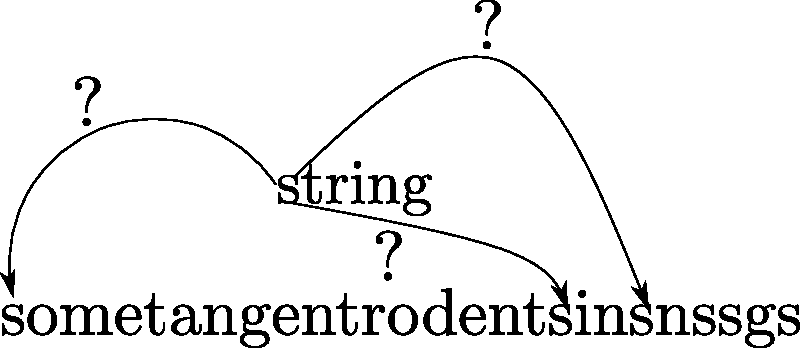
\includegraphics[scale=0.5]{figs/example-greedy}
  \caption{Example of decision.}
  \label{fig:gre}
\end{figure}
%
In this manner, as multiple instances of this character can be found in the
\texttt{encoded} string an important decision has to be realized in order to
decide at each step of the algorithm.
%
Therefore, the greedy strategy is \textit{choose the first instance of that
  character in the encoded string}. This is really intuitive as any forward
instance of this character just crops characters before them and could mislead
to think that the string is not encoded. Furthermore, if using any forward
character does not affect the output of the solution then selecting the first
one does not affect it either.

Taking this into account the final algorithm is given by the following code:
\code{8}{19}

\section{Solution Space}
The solution space is given by all the non-empty strings. In this manner, in the
worst case scenario the algorithm should evaluate all the characters of the
string \texttt{encoded}. This occurs when the string is not a subsequence.

Hence, if $l = \abs{\texttt{encoded}}$, with $\abs{\cdot}$ the function that
returns the length of any string, then in the worst case scenario $l$
evaluations have to be done in order to perform the algorithm.

\end{document}
